\chapter{Metodologia}
\label{chap:meto}
\begin{flushright}
	"Nada é permanente, exceto a mudança." \\
	\ \\
<<<<<<< HEAD
	(Heráclito)
\end{flushright}

Na primeira etapa fora realizado um levantamento de referências que tratam das metodologias pedagógicas e seu histórico, abordando desde as pedagogias iniciais, como tratadas por \cite{larchert}, e como exemplo as pedagogias Tradicional e Renovada, até metodologias de ensino mais atualmente aplicadas no ensino de robótica, como tratada por \cite{Dillen}, e exemplificando, o PBL (do inglês Project-based Learning) e a TBL (do inglês Team-based Learning).

A partir deste estudo, a metodologia apresentada pelo projeto Learnbotics foi proveniente de uma correlação entre as metodologias estudadas com o intuito de propor uma nova abordagem ao problema em questão, que perpassa por entre os métodos mais atuais de ensino aplicado à robótica, porém não ignorando a grande
contribuição que métodos mais clássicos podem vir a apresentar.

A abordagem apresentada será baseada em uma junção de conceitos desenvolvidos por metodologias de ensino mais voltadas para o aprendizado prático, principalmente o movimento maker, como tratado por \cite{Dillen}, atrelados a concepções de Vigotsky de propor ao aluno atividades práticas a fim de construir o conhecimento correlacionando atividades práticas e teóricas, como tratado por \cite{Palangana}.

Pode-se citar também PBL, associada a metodologias mais clássicas e teóricas, como por exemplo a pedagogia Tecnicista, e usará ainda proposição de ações baseadas em métodos considerados informais como o DIY (do inglês Do It Yourself), tratado por \cite{wolf} e fora influenciada diretamente pelo proposto pelos precursores do movimento STEM (do inglês Science, Technology, Engineering and Mathematics), como tratado por \cite{pugli}.

\begin{figure}[h!]												
	\centering		
	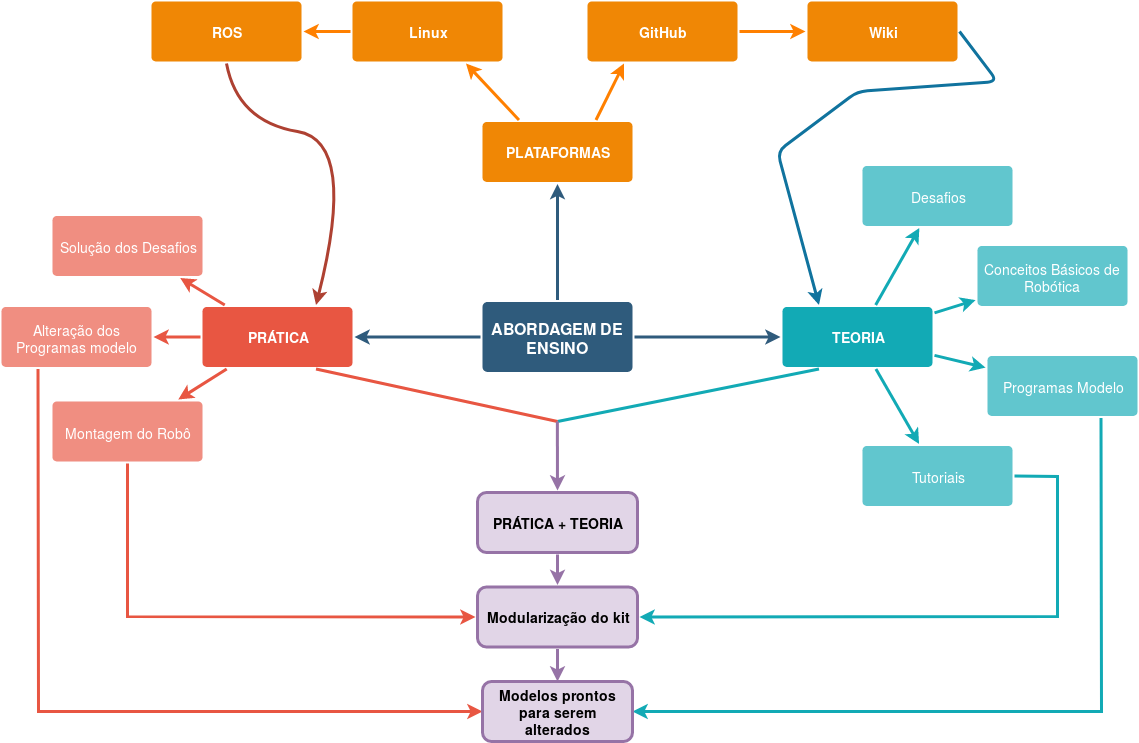
\includegraphics[width=0.5\textwidth]{Rep_graf_metodo.PNG}			
	\caption{Representação Gráfica da Metodologia}		
	\label{img:rep_metod}	
	\source{Autores, 2019}		
\end{figure}

A proposta de desenvolvimento será baseada na figura~\ref{img:rep_metod} abaixo, que apresenta os macro itens envolvidos, assim como uma exemplificação de como essas informações serão apresentadas ao estudante. 

Estes macro itens são subdivididos da seguinte maneira: Na parte teórica serão apresentados ao estudante conceitos básicos de robótica, baseados nas principais bibliografias e documentos que são normalmente utilizados pela comunidade de robótica, e já na parte prática, o aluno contará com um kit físico para ajudar a absorção dos conteúdos apresentados.

Do ponto de vista teórico, um exemplo do que será disponibilizado são os tutoriais do Framework ROS (do inglês Robot Operating System), que são elaborados pela própria comunidade do ROS. Todavia, não existem versões escritas em português, ou em uma linguagem que se preocupe em ser simplificada, o que dificulta o acesso à essas informações. Assim, a proposta é de utilizar estes tutoriais como inspiração e referência de conteúdo para produção de material escrito em linguagem mais acessível e em português.

Além da produção de tutoriais, há ainda a proposta de apresentar scripts modelo, escritos em python, que servirão como base para explicações de conceitos
de programação. O foco destes, será de mostrar aos alunos como utilizar métodos e funções próprias do framework. Estes scripts estarão envolvidos diretamente com outro macro item, que é o aprendizado prático. A parte prática tem como foco o estudo e a alteração dos scripts, proporcionando assim o desenvolvimento do estudante em programação.

Cada script modelo estará atrelado a um desafio. Para que o estudante solucione estes desafios, a proposta é que ele leia, interprete e altere o programa
para realizar uma tarefa específica que vai um pouco além da apresentada pelo script original.

Visando dar forma e visual à conceitos muitas vezes abstratos, o que é interessante na abordagem, é que, atrelado a essas alterações haverão dispositivos
reais para demonstrar se houve ou não êxito. Alguns exemplos de dispositivos com os quais os estudantes poderão interagir são servomotores e uma câmera, o que
facilitará uma absorção dos conceitos apresentados.
Para alcançar estes objetivos de aliar as macro áreas, o estudante terá contato também com uma plataforma online, o GitHub, onde encontrará todos os tutoriais e materiais complementares desenvolvidos.

Paralelo à isso, na parte física, o estudante também terá um kit físico para montagem gradual de um robô com movimentação diferencial. Esta montagem será modular e será regida pelo seu andamento nos tutoriais. O quadro~\ref{tab:quad01} apresenta os componentes presentes no kit.

% Please add the following required packages to your document preamble:
% \usepackage{graphicx}
\begin{table}[]
	\centering
	\caption{Relação dos Componentes Presentes no Kit Físico.}
	\label{tab:quad01}
	\resizebox{\textwidth}{!}{%
		\begin{tabular}{cccccccc}
			\textbf{Componentes} & \begin{tabular}[c]{@{}c@{}}Raspberry \\ Pi 3b\end{tabular} & \begin{tabular}[c]{@{}c@{}}Dynamixel \\ MX-28\end{tabular} & \begin{tabular}[c]{@{}c@{}}Câmera \\ RGB\end{tabular} & \begin{tabular}[c]{@{}c@{}}Rodas \\ Emborrachadas\end{tabular} & \begin{tabular}[c]{@{}c@{}}Roda \\ de Apoio\end{tabular} & \begin{tabular}[c]{@{}c@{}}Cabos \\ e Conexões\end{tabular} & Bateria \\
			\textbf{Quantidade}  & 1                                                            & 2                                                             & 1                                                        & 2                                                                 & 1                                                           & x                                                              & 1      
		\end{tabular}%
	}
\end{table}

A escolha da Raspberry Pi 3.0B se deve por conta da alta disponibilidade no mercado, por apresentar um custo baixo se comparado com outros computadores que serviriam para a mesma finalidade, e principalmente por apresentar poder computacional suficiente para o funcionamento do ROS e das bibliotecas de processamento de imagens que serão utilizadas.

Na Raspberry Pi será utilizado o sistema operacional Raspbian por ser o mais otimizado para a plataforma, por ser derivado de um sistema Linux, e por funcionar
aliado ao ROS Kinetic, que é hoje a distribuição do ROS mais utilizada pela comunidade da robótica.

O estudante irá receber a Raspberry com todas as bibliotecas necessárias para funcionamento e alteração dos scripts já instaladas, assim como o framework também já instalado, poupando assim o desestímulo inicial que tende a ocorrer no primeiro contato com estas ferramentas.

Serão apresentados os servomotores Dynamixel, por serem amplamente utilizados em projetos robóticos de inovação. Isso ocorre por conta da maior facilidade de integrar estes servos com o ROS, sem precisar utilizar ferramentas mais complexas, como desenvolvimento de drivers e controle PWM (do inglês, Pulse Width Modulation). Em um dos scripts modelo, por exemplo, irá ser apresentada a forma de se comunicar com os servos, juntamente à introdução da cinemática de robôs diferenciais.

A câmera RGB será utilizada para facilitar a introdução de conceitos de visão computacional e suas ferramentas, como a biblioteca do OpenCV (do inglês, Open Computer Vision). Haverão scripts modelo apresentando a integração entre ROS e OpenCV, além da proposição de desafios utilizando conceitos básicos de visão computacional. 

Ao final deste módulo, será apresentado para o estudante o desafio final do kit, que se tratará de uma integração dos conhecimentos apresentados previamente.
=======
	(Gandalf)
\end{flushright}

\section{Metodologia de Ensino}\label{sec:metod_ensino}
Visando facilitar a implementação e integração do ensino de robótica no Brasil, foi desenvolvido um kit de robótica pedagógica para ser aplicado em ambientes educacionais e extrapolar os limites da sala de aula, permitindo que os conceitos de robótica possam ser aprendidos pelos entusiastas em qualquer ambiente. A metodologia de ensino foi baseada nos requisitos fundamentais de robótica educacional, a fim de proporcionar aos alunos momentos de aprendizado, lazer e entretenimento. Para tal, foi realizado um estudo das principais e mais eficazes didáticas de ensino de robótica ao redor do mundo, a fim de reunir os métodos mais utilizados e comprovadamente efetivos para aplicar no projeto. Desta maneira, foram selecionadas as seguintes metodologias de aprendizado: o aluno deve ser motivado a desenvolver pensamento crítico, analisar soluções e superar desafios através da metodologia PBL; o kit de aprendizado pode ser utilizado e montado em equipe para propiciar o aprendizado coletivo e o desenvolvimento de virtudes como união e trabalho em equipe, características fundamentais para os profissionais do futuro, através da metodologia TBL; a metodologia DIY está presente permitindo que qualquer pessoa possa se interessar e aprender com as próprias ações sem precisar de um ambiente escolar ou de um professor; e a participação no movimento maker ao desmistificar o mundo da robótica e atrair novos entusiastas através de linguagem simples e atrativa. De todos os trabalhos mais relevantes na área de ensino de robótica, ao menos duas das características selecionadas para o projeto estavam presentes.
	
>>>>>>> metod
